\documentclass{beamer}
\usepackage{caption}
\usepackage{wrapfig}
\usepackage[parfill]{parskip}
\usepackage{amsfonts}
\usepackage{braket}

% For more themes, color themes and font themes, see:
% http://deic.uab.es/~iblanes/beamer_gallery/index_by_theme.html
%
\mode<presentation>
{
  \usetheme{CambridgeUS}       % or try default, Darmstadt, Warsaw, ...
  \usecolortheme{default} % or try albatross, beaver, crane, ...
  \usefonttheme{serif}    % or try default, structurebold, ...
  \setbeamertemplate{navigation symbols}{}
  \setbeamertemplate{caption}[numbered]
} 

\usepackage[english]{babel}
\usepackage[utf8x]{inputenc}
\usepackage{chemfig}
\usepackage[version=3]{mhchem}
\usepackage{braket}
\definecolor{darkred}{rgb}{0.8,0,0}
\definecolor{Blue}{rgb}{0.2,0.2,0.7}
% On Overleaf, these lines give you sharper preview images.
% You might want to `comment them out before you export, though.
\usepackage{pgfpages}
\pgfpagesuselayout{resize to}[%
  physical paper width=8in, physical paper height=6in]

\def\bone{\mathbf{1}}
\def\b0{\mathbf{0}}
\def\bx{\mathbf{x}}
\def\by{\mathbf{y}}
\def\bz{\mathbf{z}}
\def\ba{\mathbf{a}}
\def\bb{\mathbf{b}}
\def\bc{\mathbf{c}}
\def\bd{\mathbf{d}}
\def\be{\mathbf{e}}
\def\bh{\mathbf{h}}
\def\bm{\mathbf{m}}
\def\bp{\mathbf{p}}
\def\bq{\mathbf{q}}
\def\br{\mathbf{r}}
\def\bs{\mathbf{s}}
\def\bft{\mathbf{t}}
\def\bv{\mathbf{v}}
\def\bg{\mathbf{g}}
\def\bk{\mathbf{k}}
\def\bu{\mathbf{u}}
\newcommand{\cF}{\mathcal{F}}
\newcommand\diff{\mathrm{d}}
\newcommand{\cG}{\mathcal{G}}
\newcommand{\Naniso}{N_{\text{aniso}}}
\newcommand{\Niso}{N_{\text{iso}}}
\def\bf{\boldsymbol}


\setbeamerfont{enumerate subbody}{size=\scriptsize}
\setbeamerfont{caption}{size=\tiny}


% Here's where the presentation starts, with the info for the title slide
\title{A Brief Introduction to Deep Learning and Computer Vision}
\author{Jacob Blum}
\institute{Department of Radiology, Washington University in St. Louis School of Medicine}
\date{\today}


\setbeamerfont{itemize/enumerate body}{size = \tiny}
\setbeamerfont{itemize/enumerate subbody}{size=\tiny} %to set the body size


\begin{document}

\begin{frame}[plain]
    \titlepage
  \end{frame}

  
% These three lines create an automatically generated table of contents.
\begin{frame}[plain]{Outline}
  \tableofcontents
\end{frame}


\section{About Me}
\begin{frame}[plain]{About Me}


    \begin{enumerate}
        \item \textbf{About:} \mbox{}\\ I am a researcher at the Mallinckrodt Institute of Radiology in Washington University in Saint Louis. I received a BA in Applied Mathematics and Statistics at WashU, advised by Sheng-Kwei Song (Radiology) and Donsub Rim (Mathematics).  \mbox{}\\ \textbf{\textit{Github: @jacobblum}}
        \item \textbf{Research Interests:} \mbox{}\\ My interests are in inverse problems and computational applications in medical imaging: coupled-physics imaging (NMR/dMRI), proton dynamics, deep learning, high performance computing.
        \item \textbf{Some Selected Publications/ Software:} 
        
        \begin{enumerate}
            \item \textbf{simDRIFT: a software package for massively parallel forward simulation of diffusion weighted MRI on biophysically accurate tissue systems} \mbox{}\\ \textit{J. Open Source Softw. (2023)}
            \item \textbf{Diffusion basis spectrum imaging provides insights into cervical spondylotic myelopathy pathology} \mbox{}\\ \textit{Neurosurgery (2022)}
            \item \textbf{Analysis of combined clinical and diffusion basis spectrum imaging metrics predicts the outcome of chronic cervical spondylotic myelopathy following cervical decompression surgery} \mbox{}\\ \textit{J. of Neurosurgery: Spine (2022)}
            \item \textbf{Diffusion Basis Spectrum Imaging Distinguishes High Grade Glioma Treatment Effect From Tumor Progression} \mbox{}\\ \textit{Neuro-Oncology (2023)}
            \item \textbf{Utility of Diffusion Basis Spectrum Imaging in Quantifying Baseline Disease Severity and Prognosis of Cervical Spondylotic Myelopathy} \mbox{}\\ \textit{Spine (2022)}
        
        
        \end{enumerate}
    \end{enumerate}
    
\end{frame}


\section{Image Processing}
\begin{frame}[plain]{What Are Images: ND-Arrays}
\begin{definition}
    Diverse mathemtaical descriptions of obejcts and images can be unifed by the imaging equation.
    \begin{align}
        \mathbf{g} = \boldsymbol{\mathcal{H}}\mathbf{f}
    \end{align}
    Where $\mathbf{g}$ is the image, $\mathbf{f}$ the imaging object, and $\mathcal{H}$ the imaging system.

    For example ...

    \begin{figure}
        \centering
            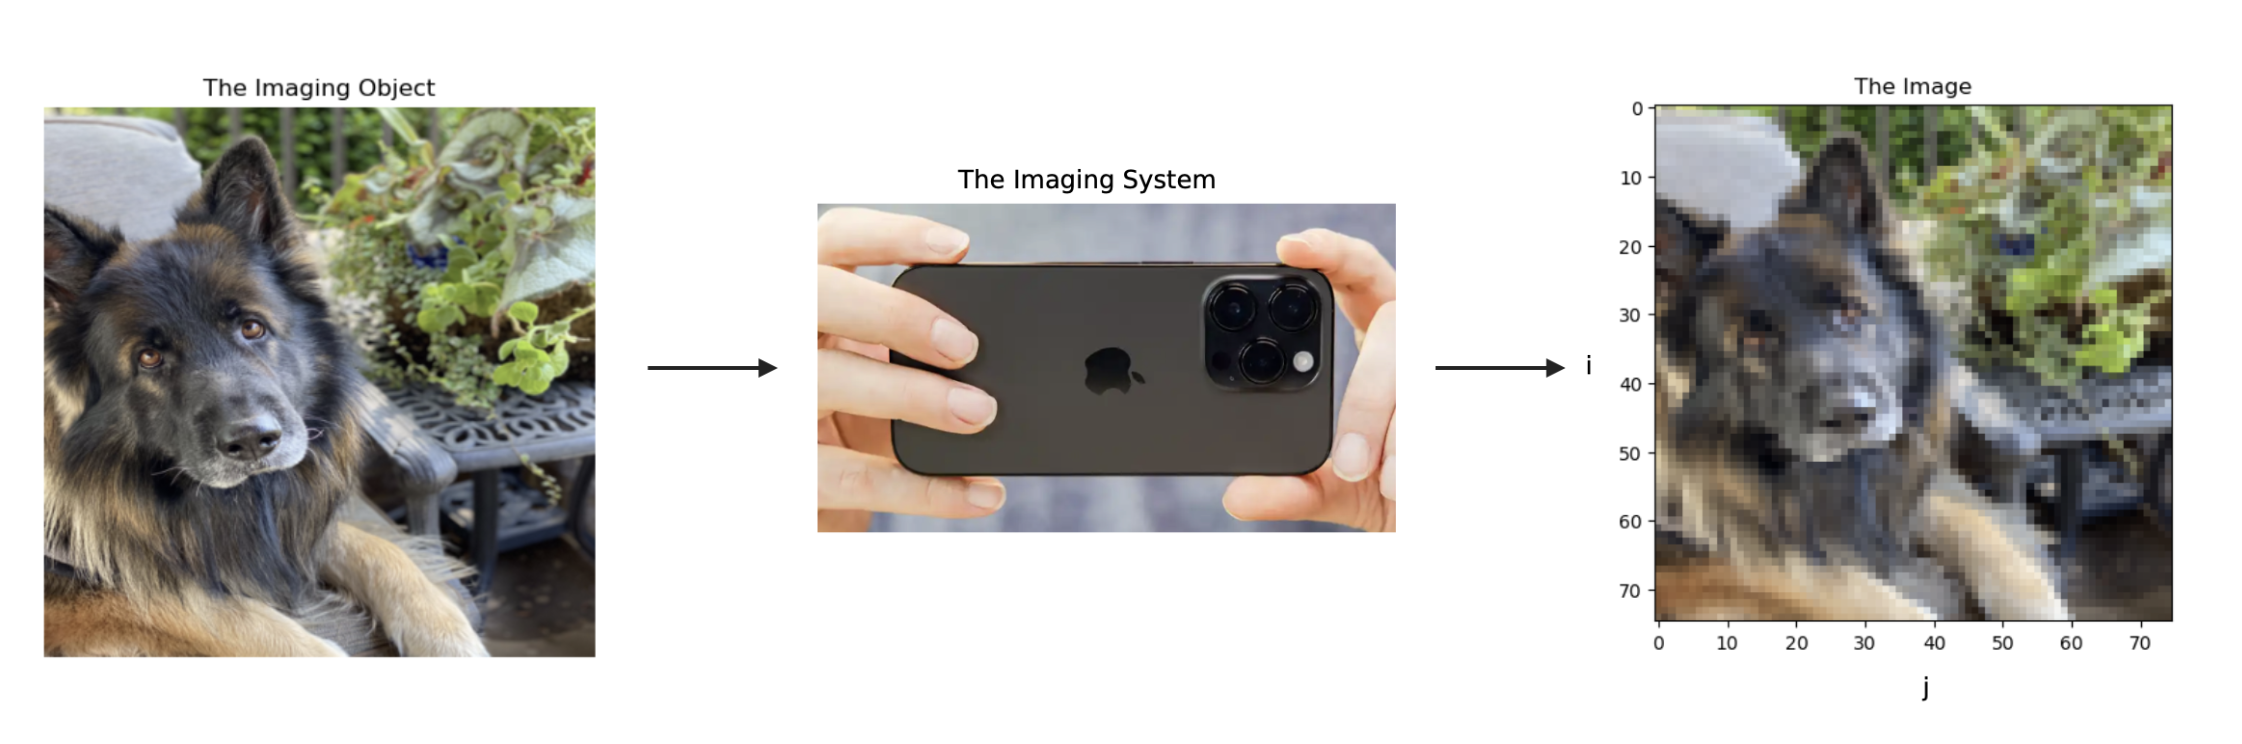
\includegraphics[width = \textwidth]{/Users/jacobblum/Desktop/cv_tex/figs/an_imaging_system.png}
            \caption{The Imaging system (a camera) produces a discretized represtnation of the imaging object. Typically, this is can be thought of as a 2D array for greyscale images or a 3D array for RGB images.}
        \end{figure}
    \end{definition}
\end{frame}

\begin{frame}[plain]{What do we do with Images: Image Processing}
    There is an enormous demand for image processing in a diverse range of application areas including biomedical imaging, autonomous systems, and remote sensing.
    \begin{figure}
        \centering
            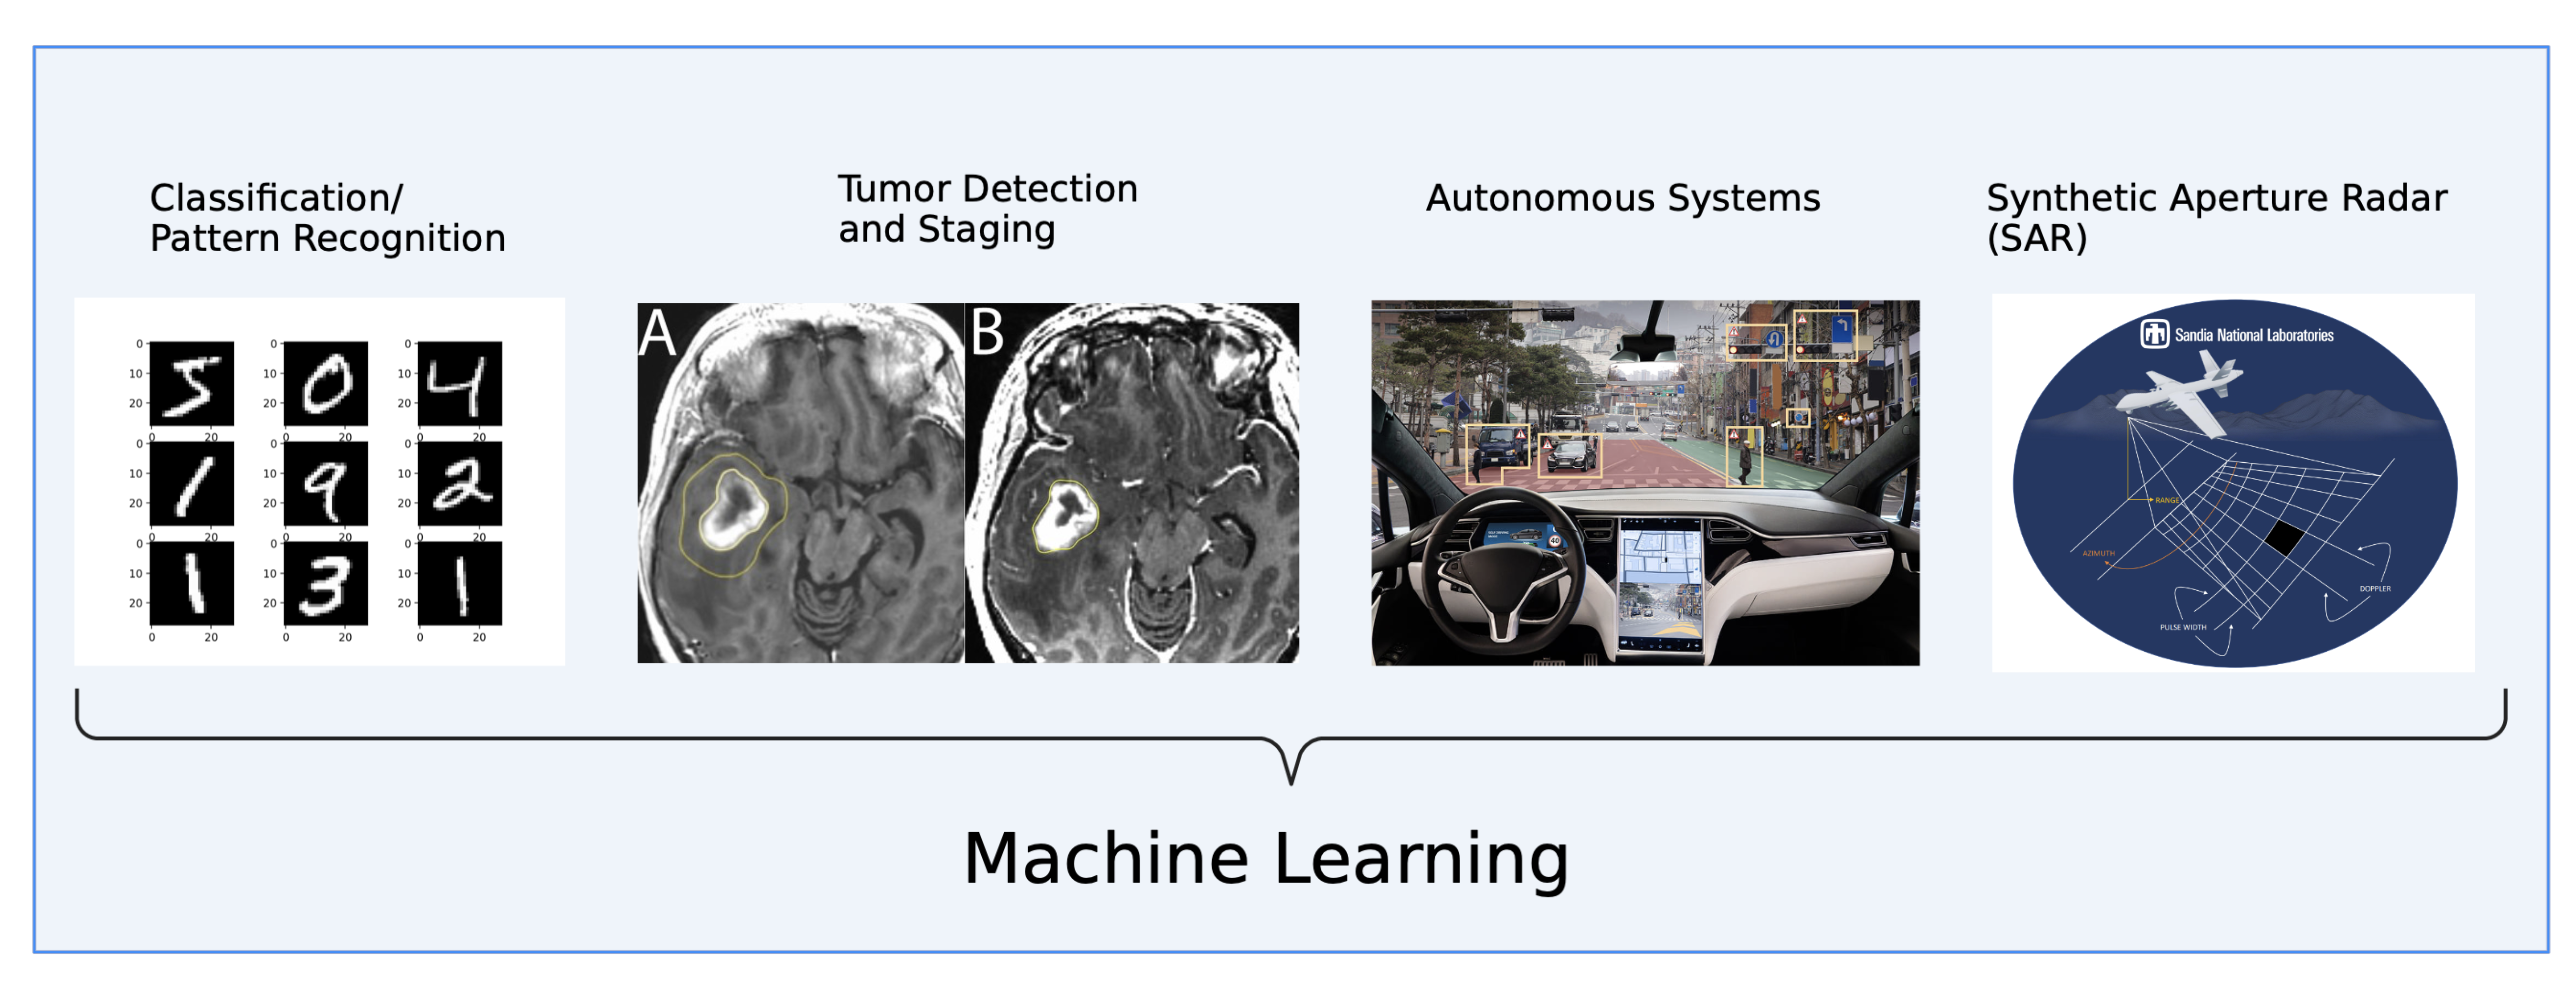
\includegraphics[width = \textwidth]{/Users/jacobblum/Desktop/cv_tex/figs/Image Processing.png}
            \caption{(Left) MNIST Dataset, a common benchmark for image classication models; T2W/FLAIR images of GBM with ML guided segmentation; A self driving car using computer vision; A SAR system on a UAV}
        \end{figure}
\end{frame}

\section{Machine Learning}

\subsection{Some Definitions}
\begin{frame}[plain]{What is Machine Learning?}
    \begin{columns}
        \begin{column}{0.45\textwidth}
            \begin{definition}{Learning Algorithm:}
                A computer program is said to learn from experince $E$ with respect to some class of tasks $T$ and performance measure $P$, 
                if its performance at tasks in $T$, as measured by $P$ improves with expeirence $E$. (Mitchell, 1997)
            \end{definition}
            
        \end{column}
        \begin{column}{0.45\textwidth}  
            \begin{figure}
                \centering
                    
\includegraphics[width = \textwidth]{/Users/jacobblum/Desktop/cv_tex/figs/what_is_dl.jpg}
                \end{figure}
        \end{column}
        \end{columns}
\end{frame}

\begin{frame}[plain]{The Task, $T$}
    Machine learning \textit{tasks} are usually described in terms of how the machine learning system should process an $\textbf{example}$. 
    
    \begin{definition}
    An example is a collection of $\textbf{features}$ that have been quantataivley measured from some object or event that we want the machine learning system to process (i.e., an image).
    \end{definition}
  
    Many kinds of tasks can be solved with machine learning. We will mainly focus on $\textbf{object recognition}$

    \begin{definition}
        \textbf{Object Recogniztion}: In this type of task, the program is asked to specify which of $k$ categories some input image belongs to. To solve this taks, the learning algorithm will produce
        a function
        \begin{align}
            f : \boldsymbol{\mathcal{H}}\mathbf{f} \mapsto \{1,...,k \}
        \end{align}
        That assigns numeric labels that identify the object in the image.
    \end{definition}
\end{frame}

\begin{frame}[plain]{The Performance Measure, $P$}
To evaluate the abilities of a machine learning algorithm, we must design a quantative measure of its performance. Usually, this performance measure $P$ is specify
to the task $T$ being carried out by the system. For classication, Binary Cross Entropy is a popular choice!

For tasks such as $\textbf{object recogniztion}$, we often measure the $\textbf{accuracy}$ of the model, which is just the proprotion of examples for which the model produces the correct output. 

Usually, we are interested in how well the machine learning algorithm performs on data that is has not seen before, since this determines how well it willwork when deployed in the real world.
We estimate this performance with a $\textbf{test set}$ of data that we seperate from the data used for training the system.
\end{frame}

\begin{frame}[plain]{The Experience, $E$}
Machine learning algorithms can be broadly categorized as $\textbf{unsupervised}$ or $\textbf{supervised}$ by what kind of experience they are allowed to have during the learning process. We will focus
on supervised leraning algorithms.

\begin{definition}
    supervised learning algorithms expereince a dataset containing features, but each example is also associated with a $\textbf{label}$ or $\textbf{target}$.
\end{definition}

\begin{figure}
    \centering
        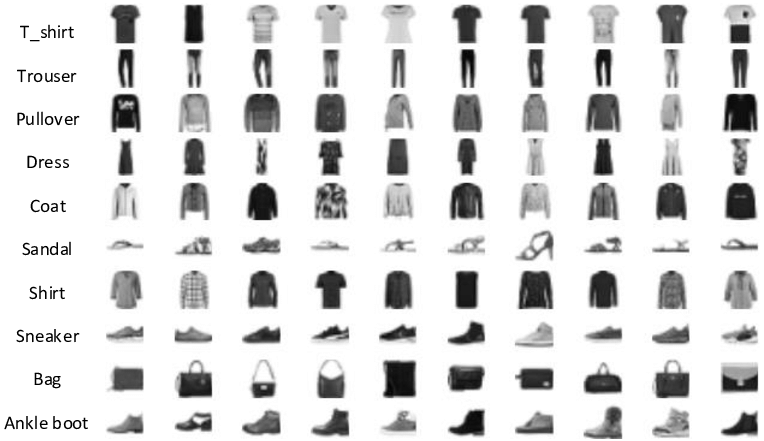
\includegraphics[width = 7cm, height = 4cm ]{/Users/jacobblum/Desktop/cv_tex/figs/fashion_MNIST.png}
        \caption{The labeled fashion-MNIST dataset, a useful benchmark for $\textbf{supervised}$ learning algorithms}
    \end{figure}
\end{frame}

\subsection{Overfitting and Underfitting}

\begin{frame}[plain]{Overfitting, and Underfitting}
\small{The central challenge in machine learning is that our algorithm must perform well on $\textit{new, previously unseen}$ inputs - not just those
on which our model was trained. The ability to perform well on previously unobserved inputs is called generalization. The factors deteriming how well a learning algorithm will perform is its ability to:}

\setbeamerfont{itemize/enumerate body}{size=\scriptsize}

\begin{enumerate}
    \item Make the training error small
    \item Mkae the gap between training the test error small
\end{enumerate}

\begin{figure}
    \centering
        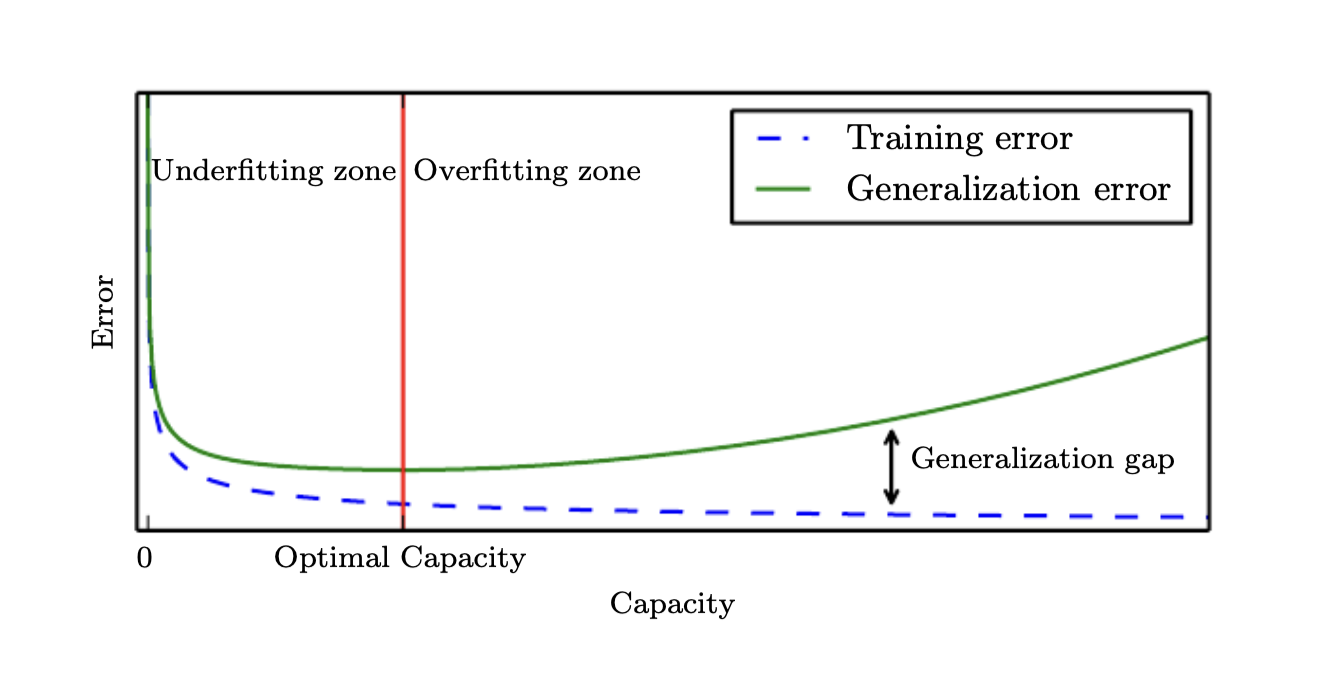
\includegraphics[width = 8cm, height = 3.8cm]{/Users/jacobblum/Desktop/cv_tex/figs/capacity.png}
        \caption{At the left end of the graph, training and generalization error are both high (Underfitting). At the right, we have 
        Overfitting, where the training error is low but the generalization gap is large. We want to avoid both scenariors.}
    \end{figure}
\end{frame}

\subsection{Optimization for Training Machine Learning Models}

\begin{frame}[plain]{Gradient-Based Optimization}
    Deep learning algorithms involve $\textbf{optimization}$ in many contexts. Typically, this is undertaken by $\textbf{gradient descent}$, an idea that traces back to Newton.
    \begin{definition}
        \small{optimization refers to the task of either minimizing or maximizing some function $f(\boldsymbol{\theta}$) by altering $\boldsymbol{\theta}$ itself.}
    \end{definition}

\begin{definition}
    \small{The gradient of a function can be thought of as a generalization of the ordinary derivative that describes the change in $f$ with respect to each of its variables. 
    It is denoted by:}
    \begin{align*}
        \nabla_{\boldsymbol{\theta}} f(\boldsymbol{\theta}) = \begin{pmatrix}
            \partial_{\boldsymbol{\theta_{1}}} f(\boldsymbol{\theta}) , \cdots \partial_{\boldsymbol{\theta}_{i-1}} f(\boldsymbol{\theta}), \partial_{\boldsymbol{\theta_{i}}} f(\boldsymbol{\theta})
        \end{pmatrix} 
    \end{align*}
    Where $\partial_{\boldsymbol{\theta}_{i}}$ is the partial derivative of $f$ with respect to $\boldsymbol{\theta_{i}}$
\end{definition}    
\end{frame}

\begin{frame}
\small{Gradient descent is based on the fact that $f(\boldsymbol{\theta})$ decreases fastest in the \textit{direction} of the negative gradeint of $f$.}
\small{Thus, gradient descent methods work by approximating the $\textbf{gradient}$, and adjusting $\boldsymbol{\theta}$ in the direction of the $\textbf{steepest descent}$.}

\begin{block}{Proof:}
\begin{align*}
    D_{\mathbf{u}} f(\boldsymbol{\theta}) = \begin{bmatrix}
        \partial_{\boldsymbol{\theta_{1}}} f(\boldsymbol{\theta}) , \cdots \partial_{\boldsymbol{\theta}_{i-1}} f(\boldsymbol{\theta}), \partial_{\boldsymbol{\theta_{i}}} f(\boldsymbol{\theta})
    \end{bmatrix} \cdot \mathbf{u} \vert_{\mathbb{S}^{n}}
\end{align*}
\begin{align*}
    D_{\mathbf{u}} f(\boldsymbol{\theta}) = | \nabla_{\boldsymbol{\theta}} | |\mathbf{u}| cos(\theta) = | \nabla_{\boldsymbol{\theta}} | cos(\theta) \qquad ( \; |\mathbf{u}| = 1 \; )
\end{align*}
Recall that $cos(\theta) \in [-1, 1]$. Thus,  $D_{\mathbf{u}} f(\boldsymbol{\theta})$ is minimizing when $\theta = \pi$. Thus, the direction of steepest
descent is $-\nabla_{\boldsymbol{\theta}}f(\boldsymbol{\theta})$! 
\end{block}
Thus, by iteratively updating $\boldsymbol{\theta}^{(i)}$ with
\begin{align*}
    \boldsymbol{\theta}^{(i+1)} = \boldsymbol{\theta}^{(i)} - \epsilon \nabla_{\boldsymbol{\theta^{(i)}}}f(\boldsymbol{\theta^{(i)}})
\end{align*}
We eventually minimize $f$!
\end{frame}

\begin{frame}[plain]{Gradient Descent in Action - A toy example}

\begin{block}{Demo:}
    \small{Let's implement and use gradeint descent to minimize the following function:}
    \begin{align*}
        f(x,y) = x^2 + y^2
    \end{align*}

    \textit{hint}:
    \begin{align*}
        \nabla_{x,y} = \begin{pmatrix}
            2x, 2y
        \end{pmatrix}
    \end{align*}
\end{block}

\begin{figure}
    \centering
        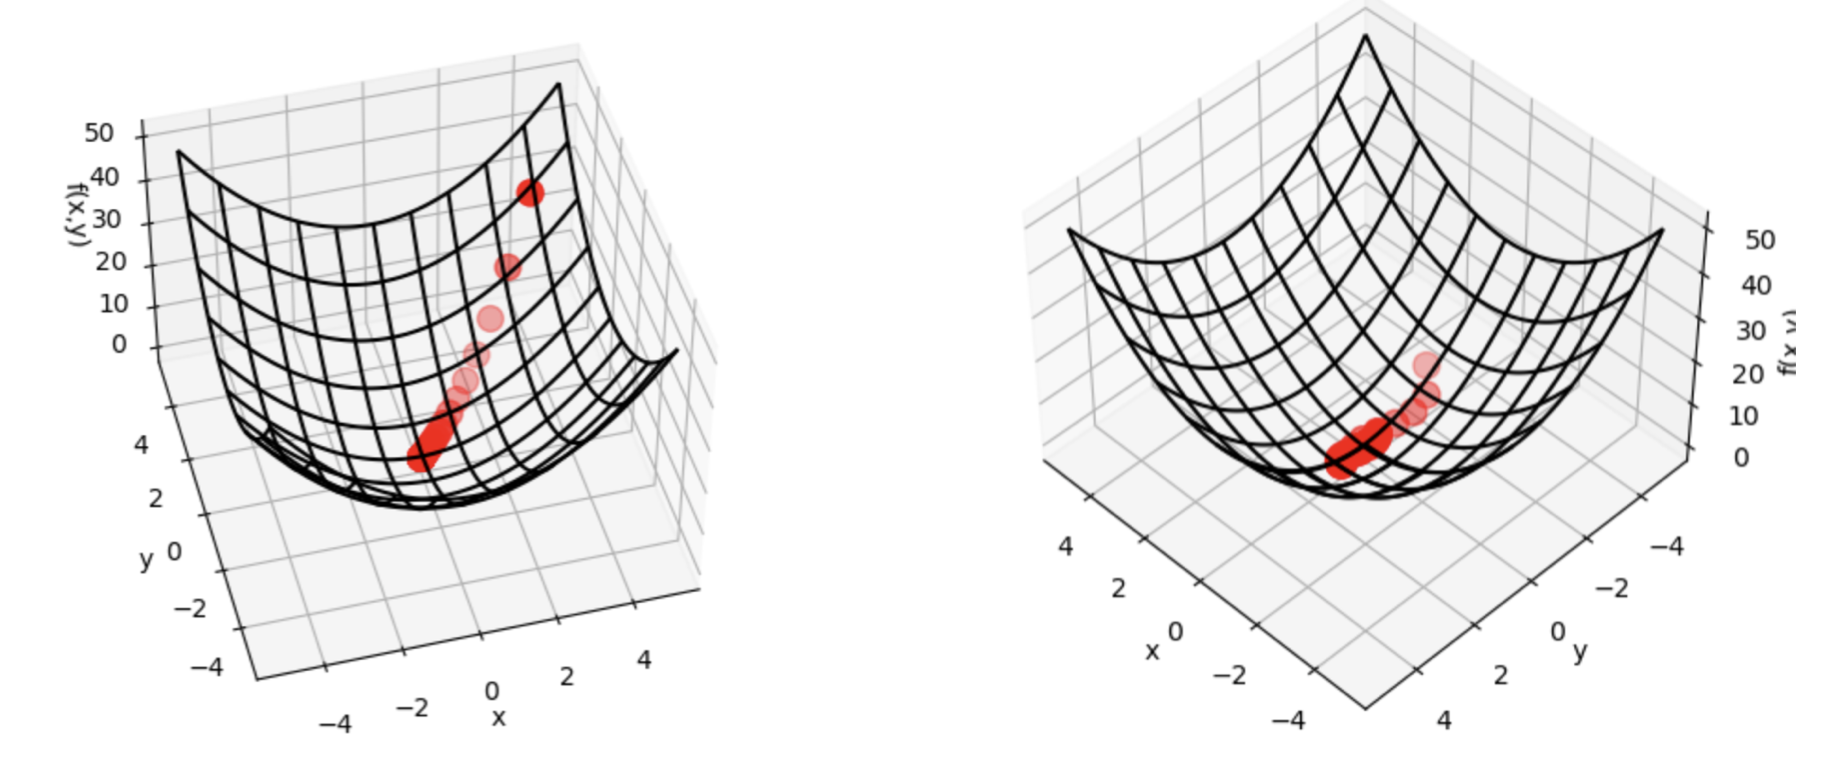
\includegraphics[width = .65\textwidth]{/Users/jacobblum/Desktop/cv_tex/figs/gd_niave_vs_pytorch.png}
        \caption{Gradient Descent minimization niave (left) vs with PyTorch (right). The advantage to using PyTorch's autograd is that we do not need 
        to know the gradient of our function, which is oftentimes the case.}
    \end{figure}
\end{frame}

\section{Modern Practical Deep Networks}
\subsection{Deep Feedforward Networks}
\begin{frame}[plain]{Deep Feedforward Networks}
    \small{$\textbf{Deep feedforward networks}$ (DNNs), also called $\textbf{multilayer perceptrons}$ (MLPs), are the quintessential deep learning model.} 

    \small{The goal of a feedforward networks is to approximate some function $f^{*}$. For example, a classifier $y = f^{*}(\mathbf{x}; \boldsymbol{\theta})$ maps an input $\mathbf{x}$ to a category $y$, and is parametized by $\boldsymbol{\theta}$!}
\begin{figure}
    \centering
    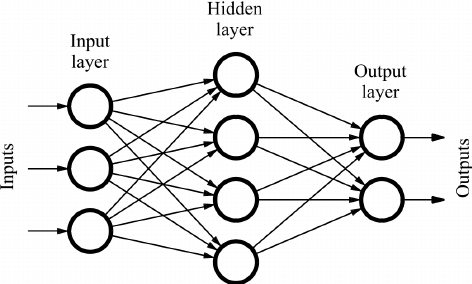
\includegraphics[width = .55\textwidth]{/Users/jacobblum/Desktop/cv_tex/figs/DNN.png}
    \caption{The diagram of a simple (1 level) feedforward neural network. Oftentimes, people use these graphs to represent the network designs. There are rich connections between
    graph theory and machine learning, particularly automatic differentiation!}
\end{figure}

\end{frame}

\begin{frame}[plain]{What's in a name?}

\begin{itemize}
    \item \small{feedforward neural networks are called $\textbf{networks}$ because they are typcially represneted by \textit{composing} together many different functions.}
           \small{For example, we might have three functions $f^{(1)}, f^{(2)}, f^{(3)}$ connected in a chain to form $f(\mathbf{x}) = f^{(3)}(f^{(2)}(f^{(1)}(\mathbf{x})))$.}

    \item \small{In this case, $f^{(1)}$ is called the $\textbf{first/input layer}$, $f^{(2)}$ is called the $\textbf{second/hidden layer}$, and so on. 
                The overall length of the chain gives the $\mathbf{depth}$ of the model, and the dimensionality of the hidden layers gives the $\mathbf{width}$. The final layer of this feedfoward network $f^{(3)}$, is called the $\textbf{output layer}$. Importantly,
                all layers in the network are connected by $\textbf{activation functions}$}

    \item \small{Finally, these networks are called \textit{neural} because they are loosely inspired by neuroscience.}
\end{itemize}
\end{frame}

\begin{frame}[plain]{Design Decisions}
    \small{The main design consideration for neural networks is deteriming the architecture, or the overall structure of the network. In chain based architectures, the main consideration
    is the $\textbf{depth}$ of the network and the $\textbf{width}$ of each layer. Typically, experimentation is required to find an optimal architecture.}
    \begin{itemize}
        \item Larger structures may perform better on certain tasks; however, are more computationally and memory expensive. 
    \end{itemize}
    \small{Yet another important consideration is the activation functions. Below are some popular choices:}
    \begin{itemize}
        \item ReLU (most popular in modern applications): $\sigma(x) = \text{max}(0, x)$
        \item sigmoid (also popular): $\sigma(x) = \frac{1}{1 + e^{-x}}$
        \item tanh: $\sigma(x) = \frac{e^{x} - e^{-x}}{e^{x} + e^{-x}}$
    \end{itemize}
    The choice of optimizer is also an important consideration:
    \begin{itemize}
        \item Adam (Most Popular and recomended)
        \item LBFGS (can perform better under specific circumstances, but is computationally expensive)
        \item Stochastic Gradient Descent (SGD) (Not necessary for the size of the data we're dealing with)
    \end{itemize}


\end{frame}
\subsubsection{Deep Neural Networks}


\begin{frame}[plain]{An Example From my research: Virtual Histology}


    \begin{columns}
        \begin{column}{0.45\textwidth}
            \begin{figure}
                \centering
                    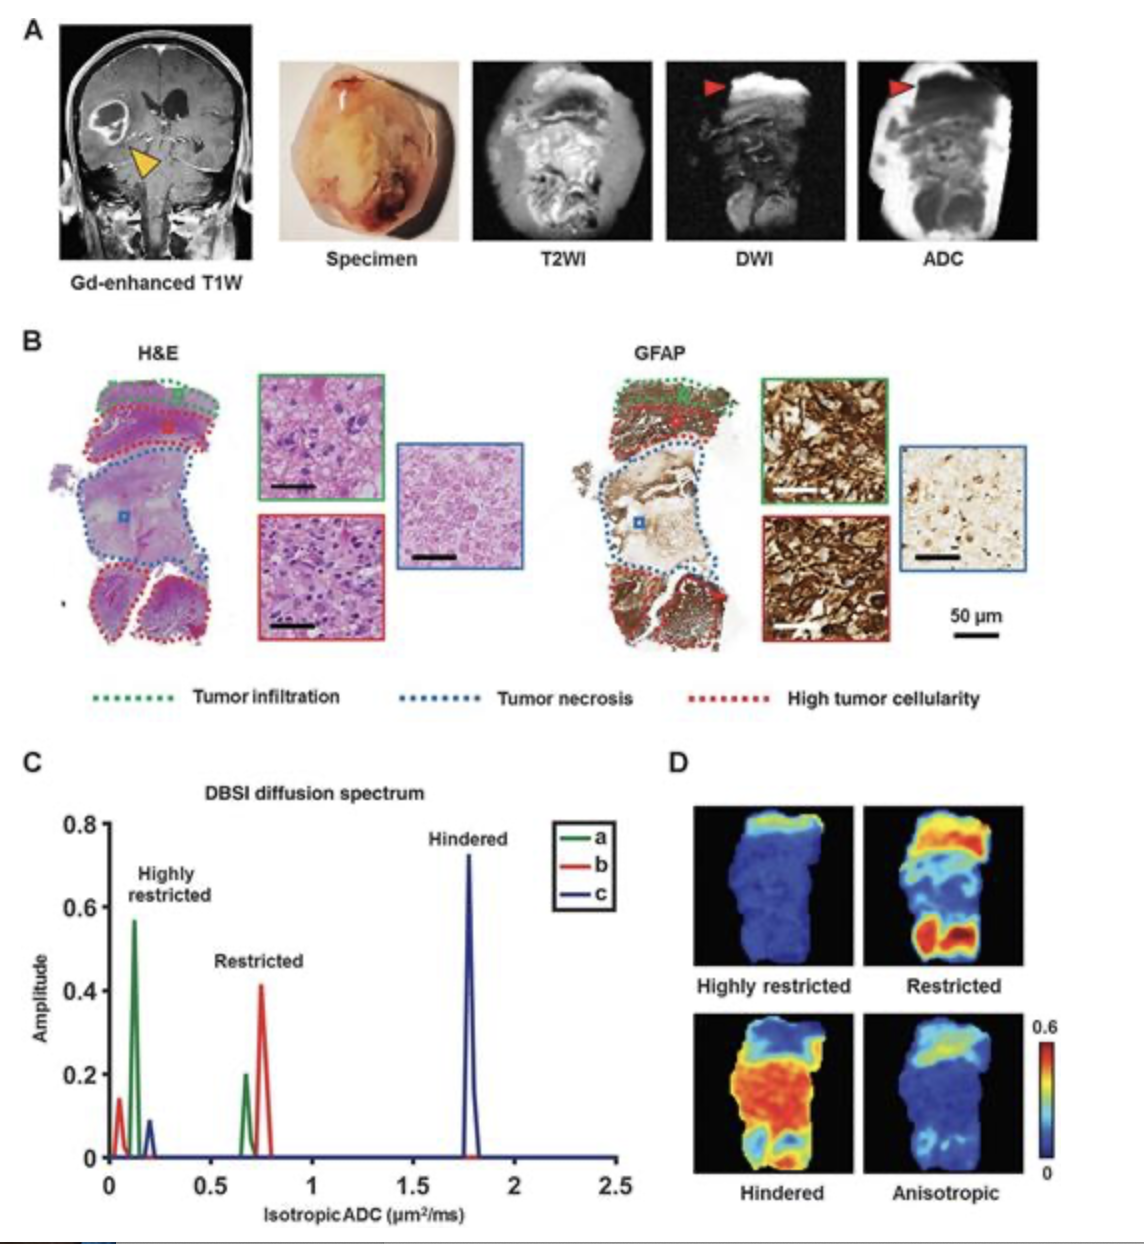
\includegraphics[width = \textwidth]{/Users/jacobblum/Desktop/cv_tex/figs/ccr_setup.png}
                \end{figure}   
        \end{column}
        \begin{column}{0.45\textwidth}  
            \begin{figure}
                \centering
                    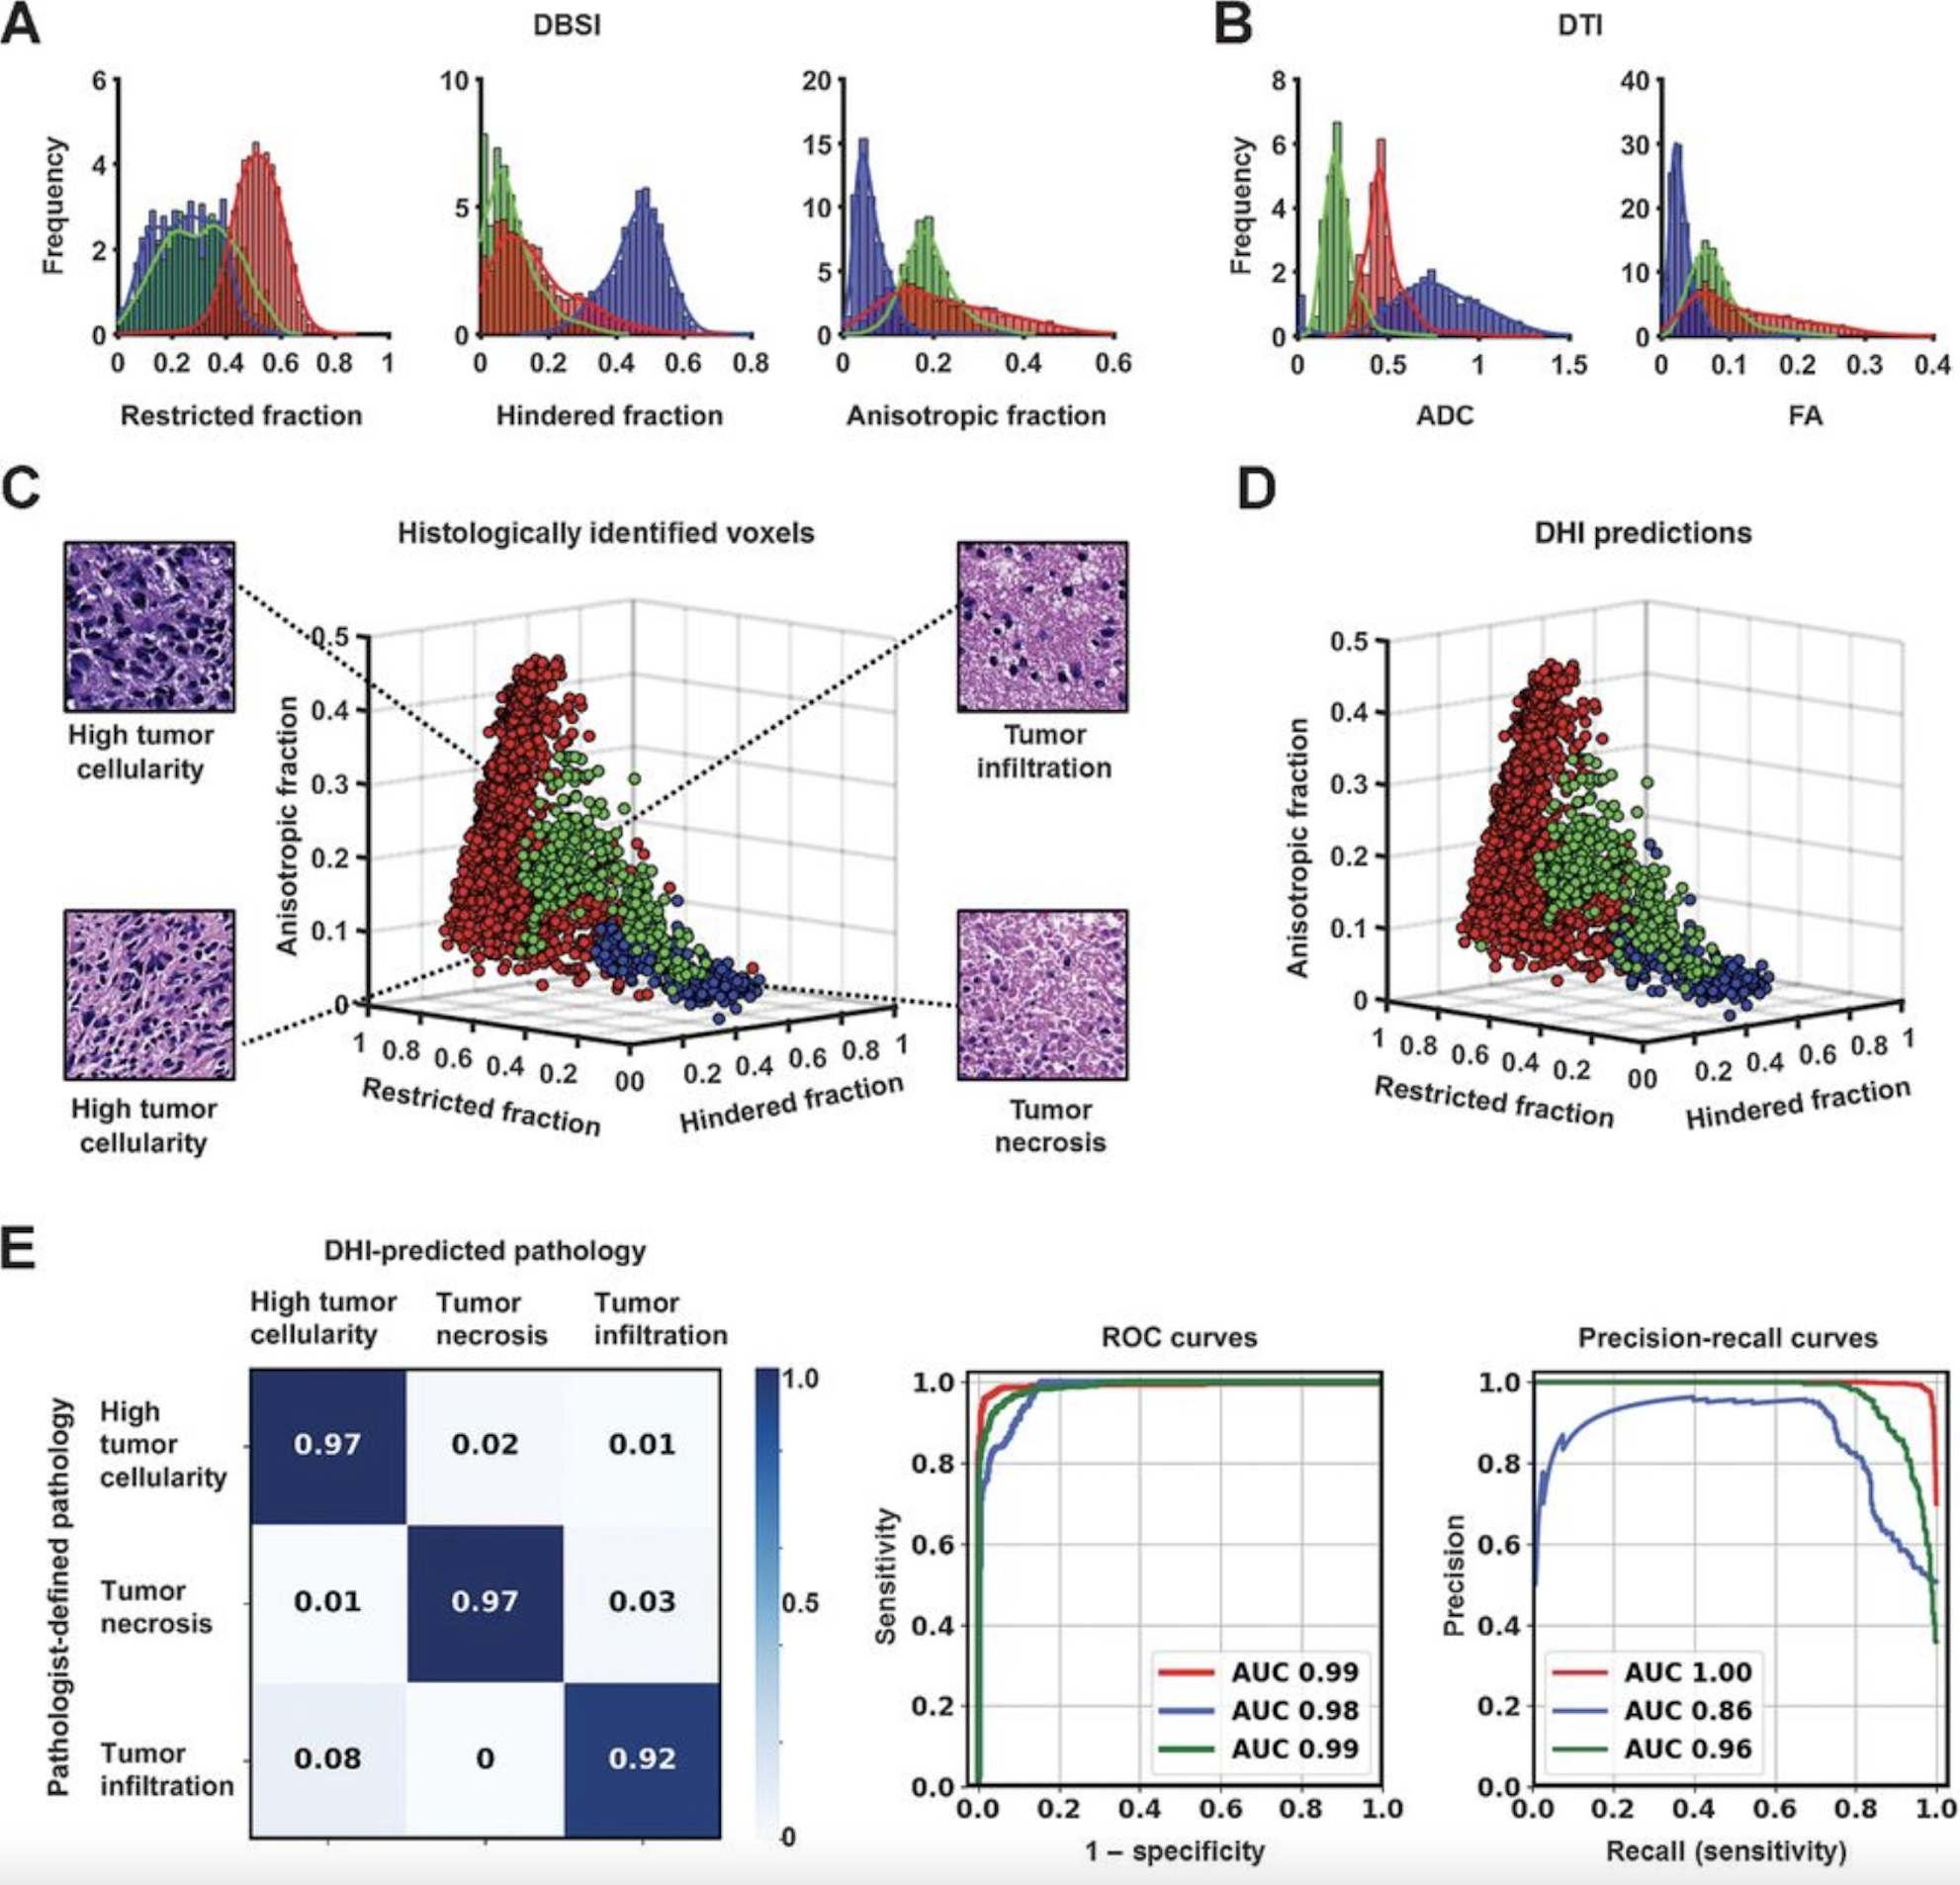
\includegraphics[width = \textwidth]{/Users/jacobblum/Desktop/cv_tex/figs/ccr_results.png}
                \end{figure}
        \end{column}
        \end{columns}



\end{frame}
\begin{frame}[plain]{Implementing a Deep Neural Network with PyTorch:}
    Workflow:
    \begin{itemize}
        \item Pick Architecture (Depth and width)
        \item Pick Activation Functions (ReLU)
        \item Pick a Task Specific loss function (Cross Entropy)
        \item Pick Optimizer (Adam)
    \end{itemize}
    \begin{figure}
        \centering
        
\includegraphics[width = .65\textwidth]{/Users/jacobblum/Desktop/cv_tex/figs/torch.png}
    \end{figure}
\end{frame}

\begin{frame}[plain]{MNIST Results}
    \begin{figure}
        \centering
        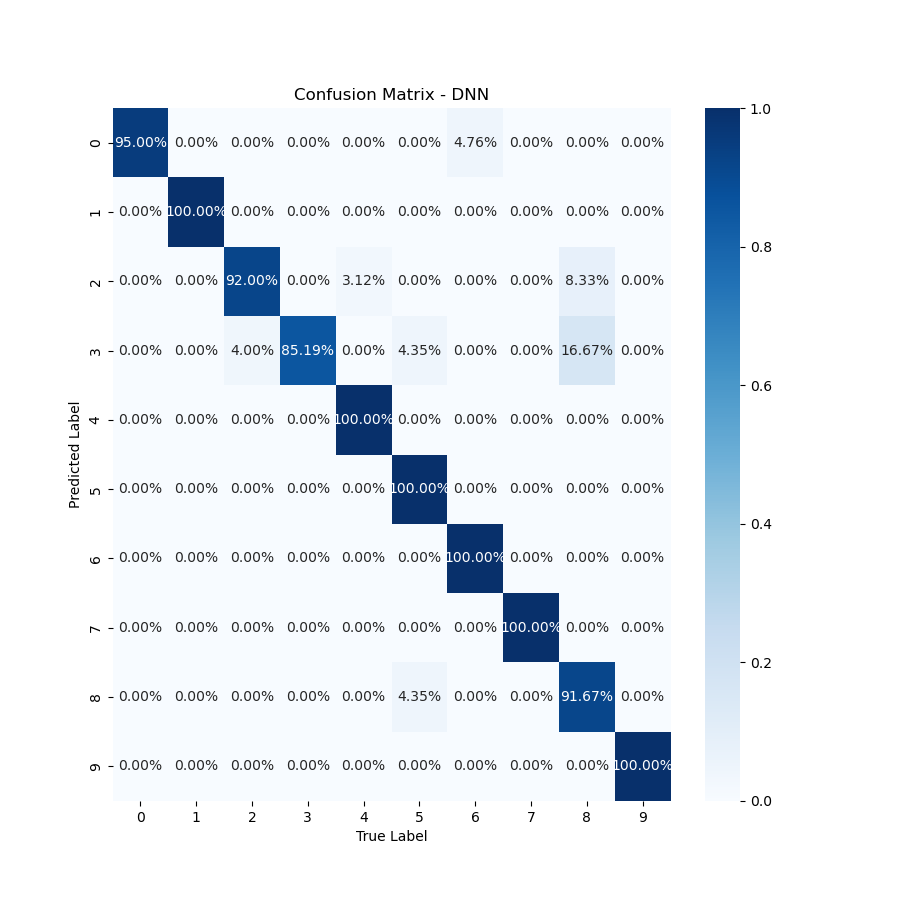
\includegraphics[width = .65\textwidth]{/Users/jacobblum/Desktop/cv_tex/figs/DNN_cm.png}
        \caption{Overall accuracy on 250 test examples : 96.79 $\%$}
    \end{figure}



\end{frame}
    

\subsubsection{Convolutional Neural Networks (CNNs)}
\begin{frame}[plain]{Convolutional Networks}
    $\textbf{Convolutional networks}$ provide a way to specialize neural networks to work with data that has a clear grid-structured topology and to scale models to very large size. This 
    approach has been most successful on two-dimensional images! 
    
    \begin{figure}
        \centering
        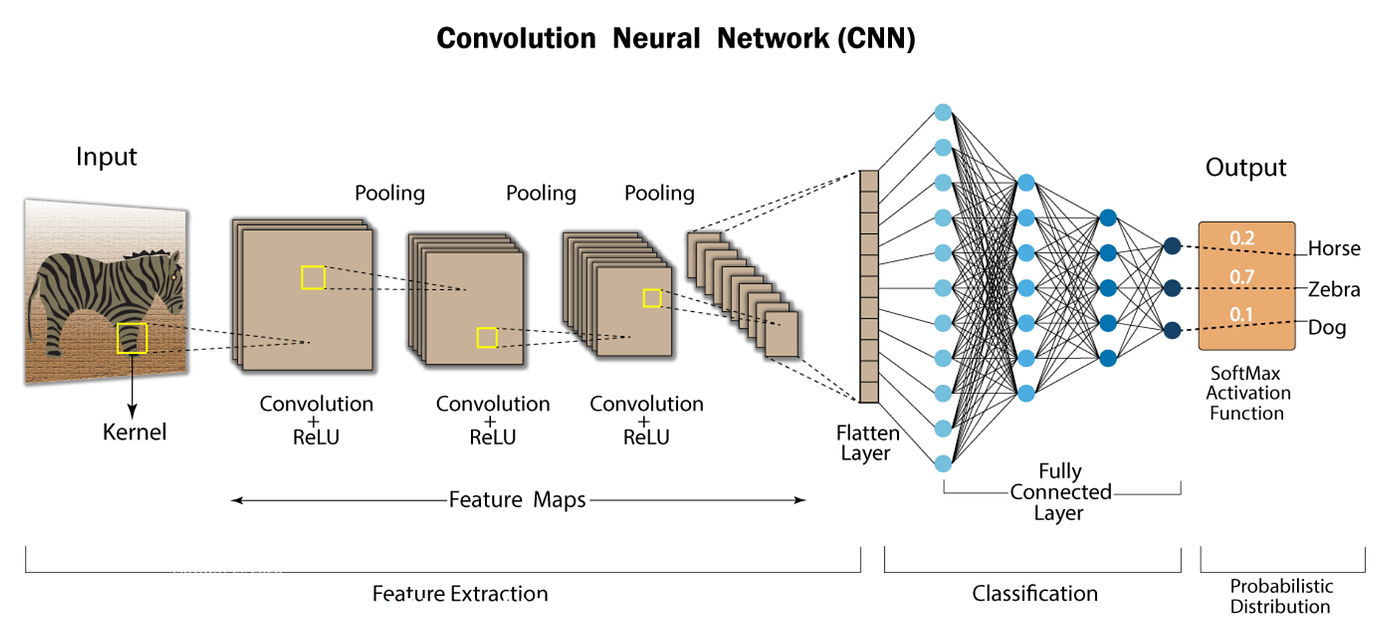
\includegraphics[width = .75\textwidth]{/Users/jacobblum/Desktop/cv_tex/figs/cnn.png}
        \caption{an example convolutional neural network (cnn) used for object recognition!}
    \end{figure}
\end{frame}

\begin{frame}[plain]{The Convolution Operation}
\begin{definition}
    $\textbf{convolution}$ is typically denoted with an asterisk
    \begin{align*}
        S(i, j) = (I * K)(i,j) = \sum_{m,n} I(m,n)K(i-m, j-n)
    \end{align*} 
    where the first argument (I) is the $\textbf{input}$ and the second is (K) is the $\textbf{kernel}$. The output is of size: $\frac{W-K+2P}{S} + 1$
\end{definition}
    \begin{figure}
        \centering
        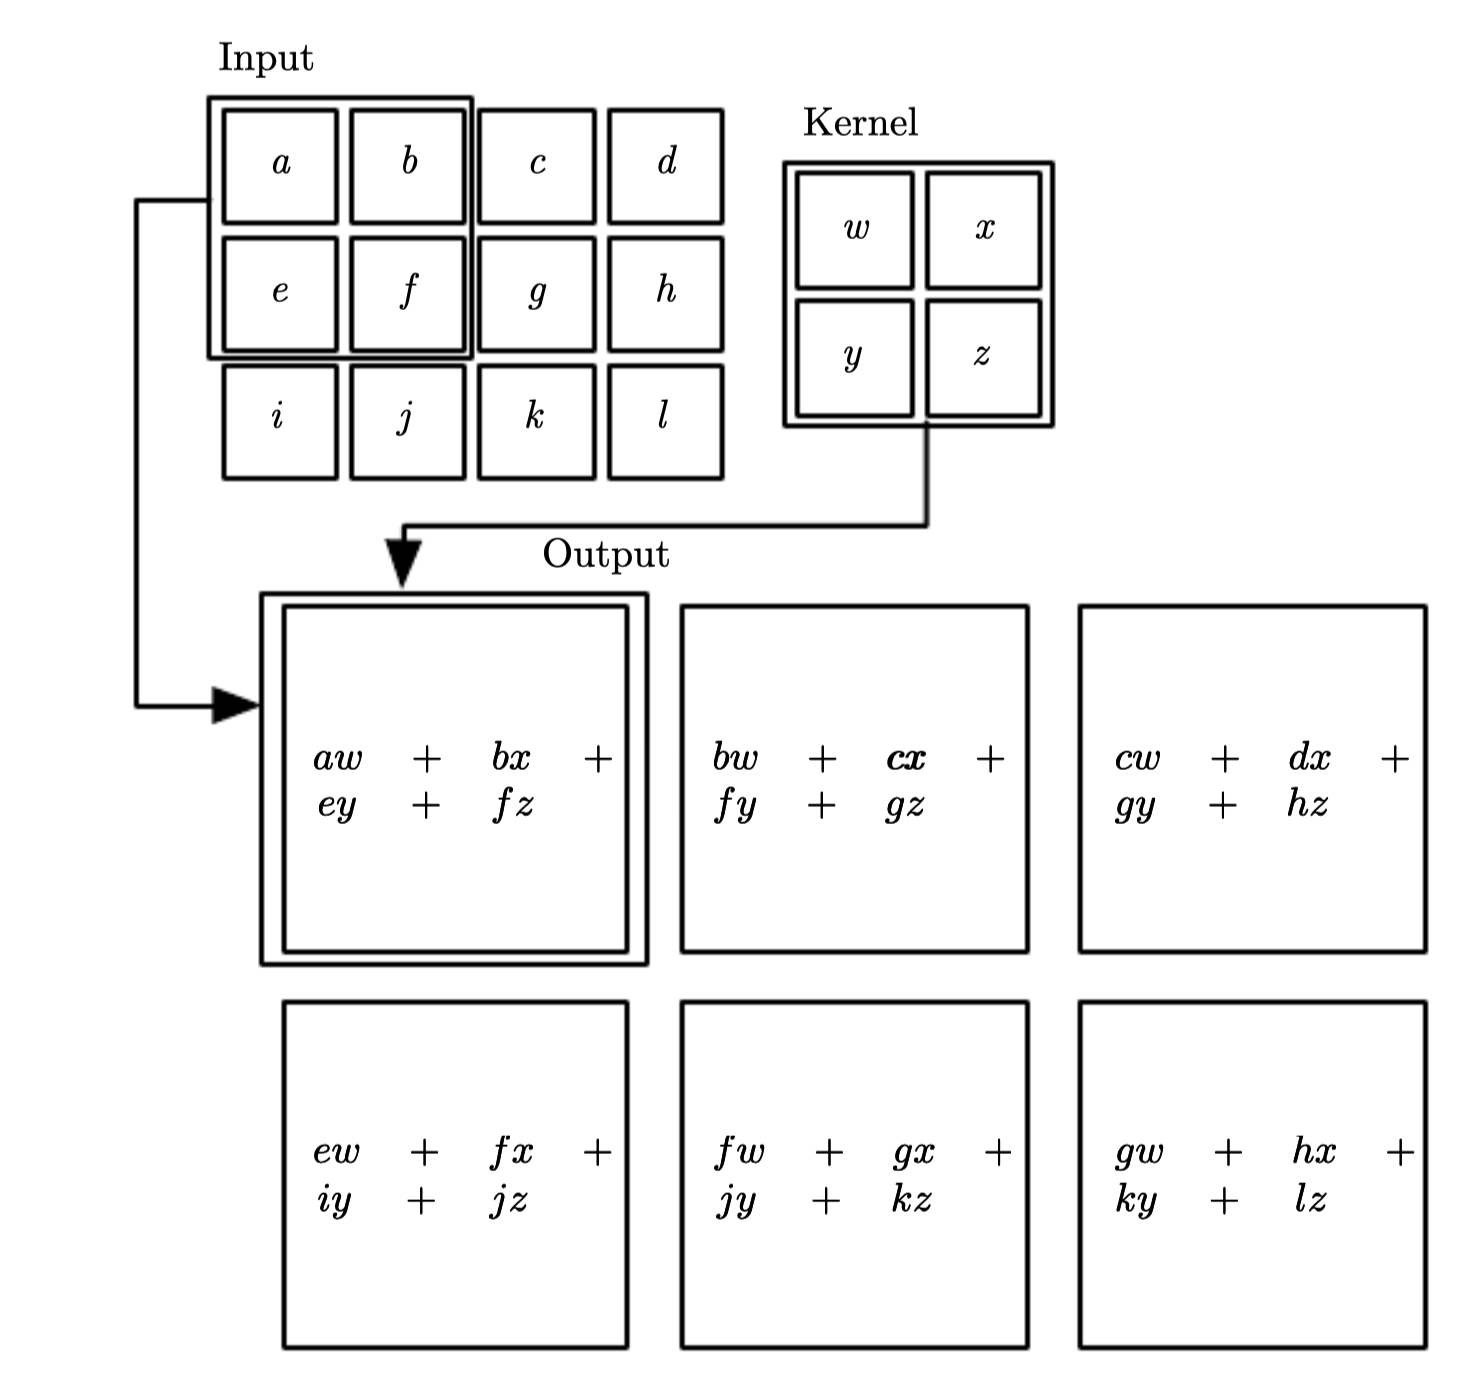
\includegraphics[width = .4\textwidth]{/Users/jacobblum/Desktop/cv_tex/figs/Screen Shot 2023-07-25 at 8.19.34 AM.png}
    \end{figure}
\end{frame}

\begin{frame}[plain]{Pooling: Learning Translational Invariance}
    \small{A typical CNN consists of three stages. In the first stage, convolution is performed. Then, the data is run through a nonlinear activation function (ReLU, for example). This is called the $\textbf{detector stage}$ In the third stage, 
    we use a $\textbf{pooling function}$ to modify the output to the layer further.} 

    \begin{figure}
        \centering
        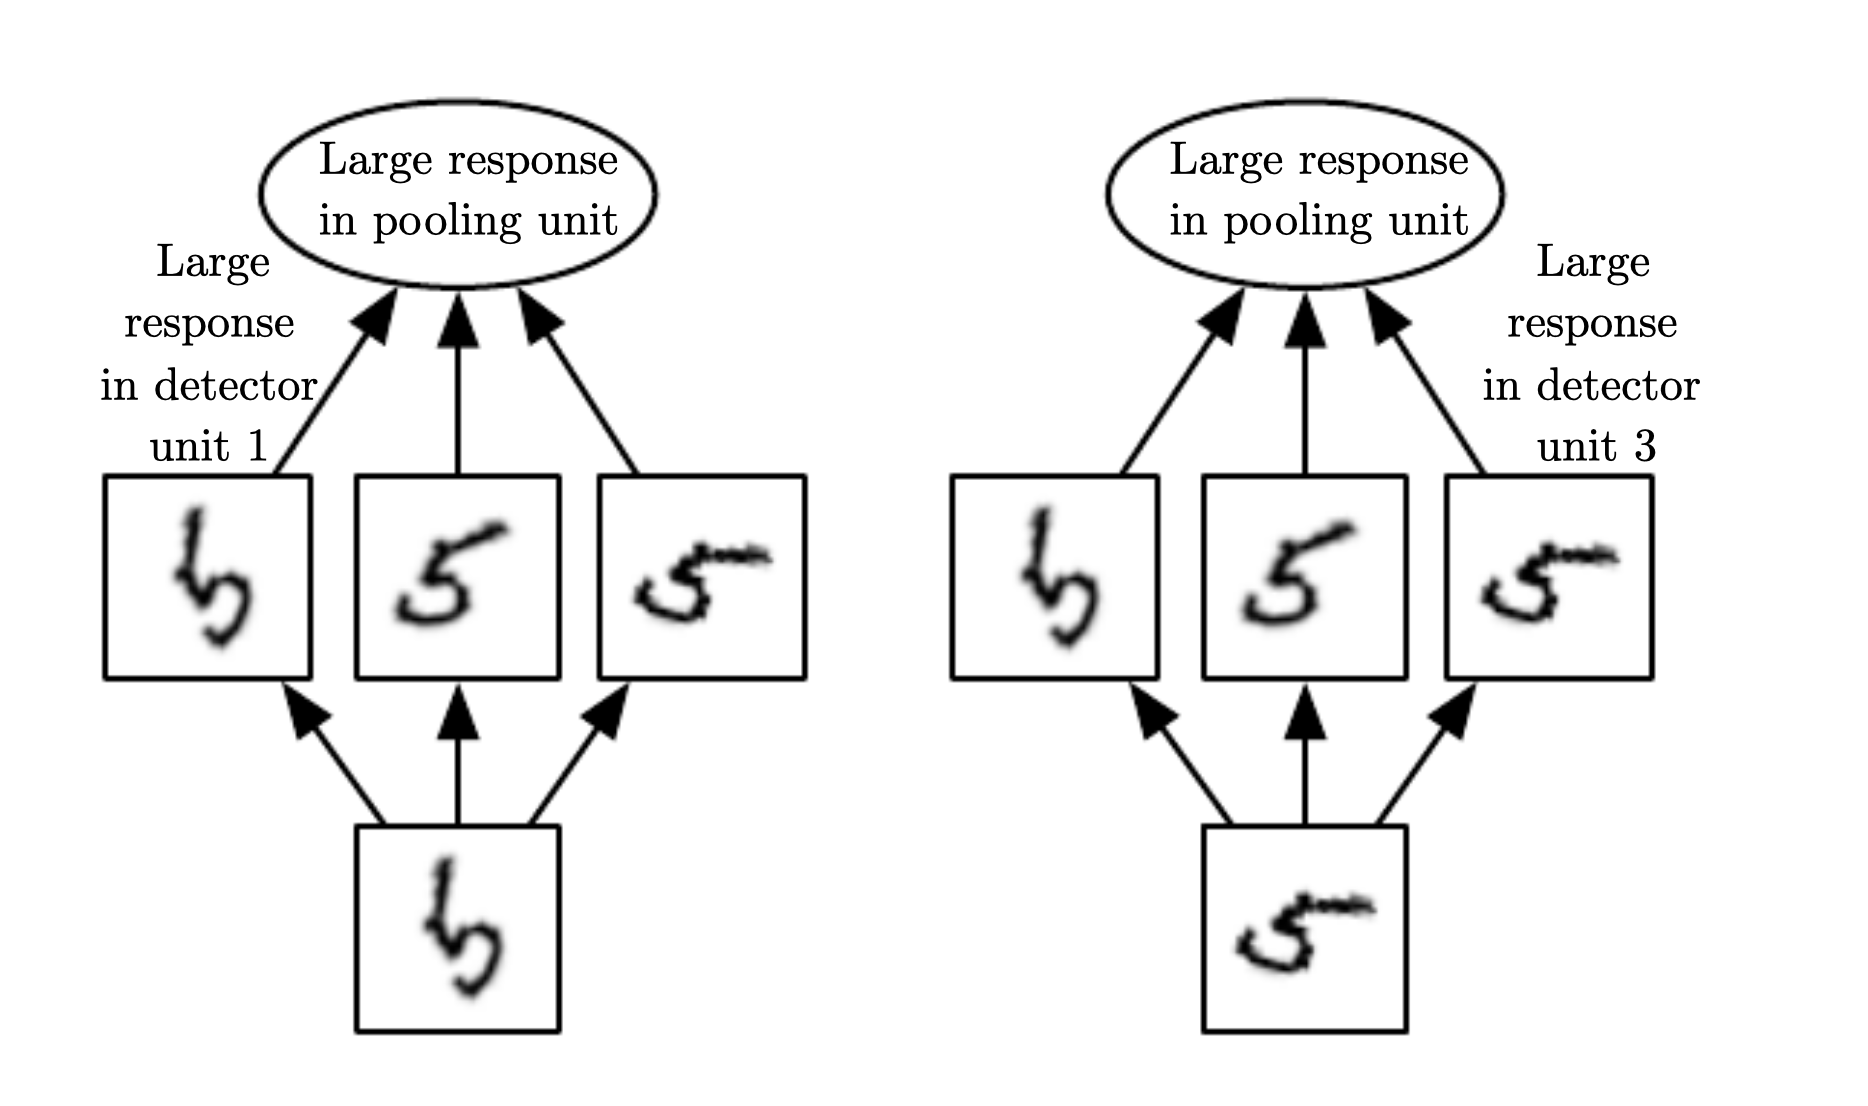
\includegraphics[width = .6\textwidth]{/Users/jacobblum/Desktop/cv_tex/figs/Screen Shot 2023-07-25 at 8.26.50 AM.png}
        \caption{A pooling unit that pools over multiple features that are learned with separate parameters is approximately $\textbf{invariant}$ to small translations of the input (rotation, scaling, etc...)
        . Here we show how a set of three learned filters and a max pooling unit can learn to become invariant to rotation. All three filters are inteded to detect a hand written 5. Each filter attamples to match a slightly differnt orientation of the 5. When a 5 appears 
        in the input, the filter will match it and cause a large activation in a detector unit. The max pooling unit then ahs a large activation regardless of which detector unit was activated!}
        
    \end{figure}

\end{frame}



\begin{frame}
    Let's see if a CNN can beat the MNIST benchmark set by the network we just implemented!
\end{frame}

\begin{frame}[plain]{MNIST Results}
    \begin{figure}
        \centering
        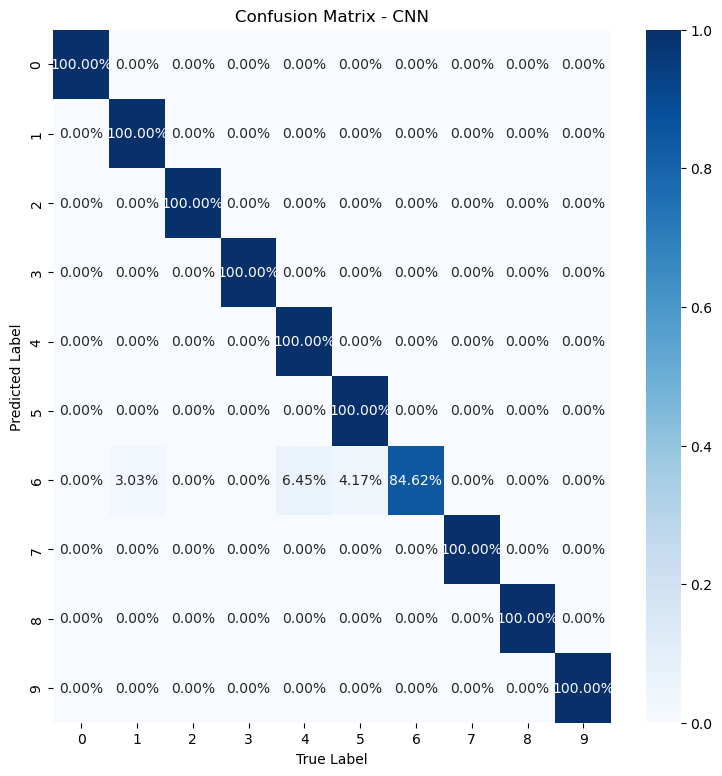
\includegraphics[width = .55\textwidth]{/Users/jacobblum/Desktop/cv_tex/figs/confusion_matrix_cnn.png}
        \caption{Overall accuracy on 250 test examples : 98.40 $\%$}
    \end{figure}
\end{frame}

\begin{frame}[plain]{Practical Considerations}
    \small{Training a CNN is prohibatively computationally expensive on a robot. Furthermore, significant effort has been dedicated to the development of accurate object detection models.}

    \begin{figure}
        \centering
        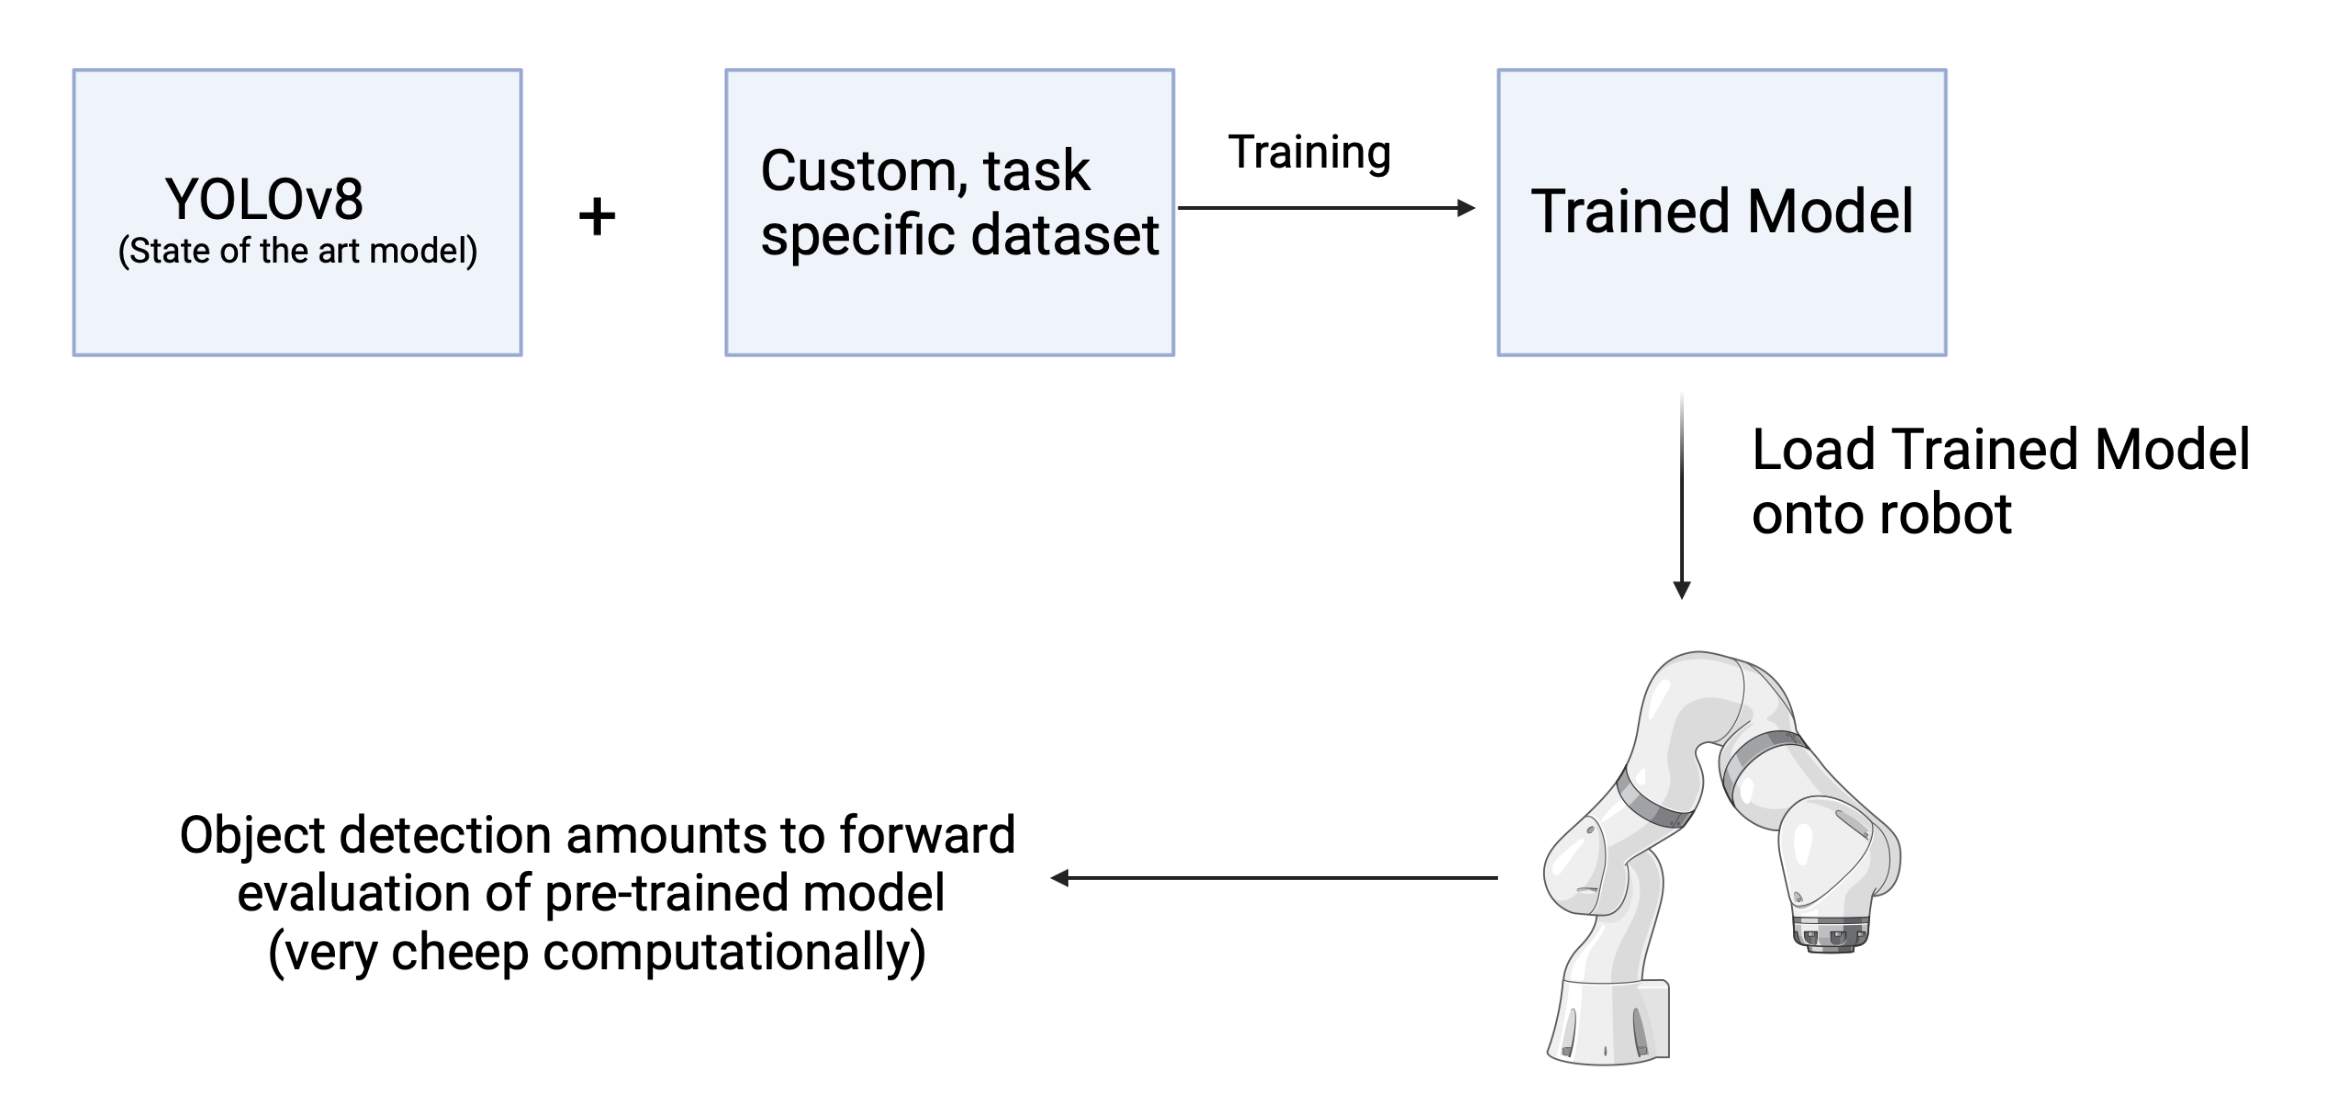
\includegraphics[width = .75\textwidth]{/Users/jacobblum/Desktop/cv_tex/figs/YOLOv8.png}
        \caption{what I would do}
    \end{figure}

    \small{Importantly, a model can only be as good as its training data. For successful object detection, the training data must be correctly labeled and sufficiently encompass 
    any type of testing scenario!}
\end{frame}

\begin{frame}[plain]{Learning About Deep Learning}
    \begin{figure}
        \centering
        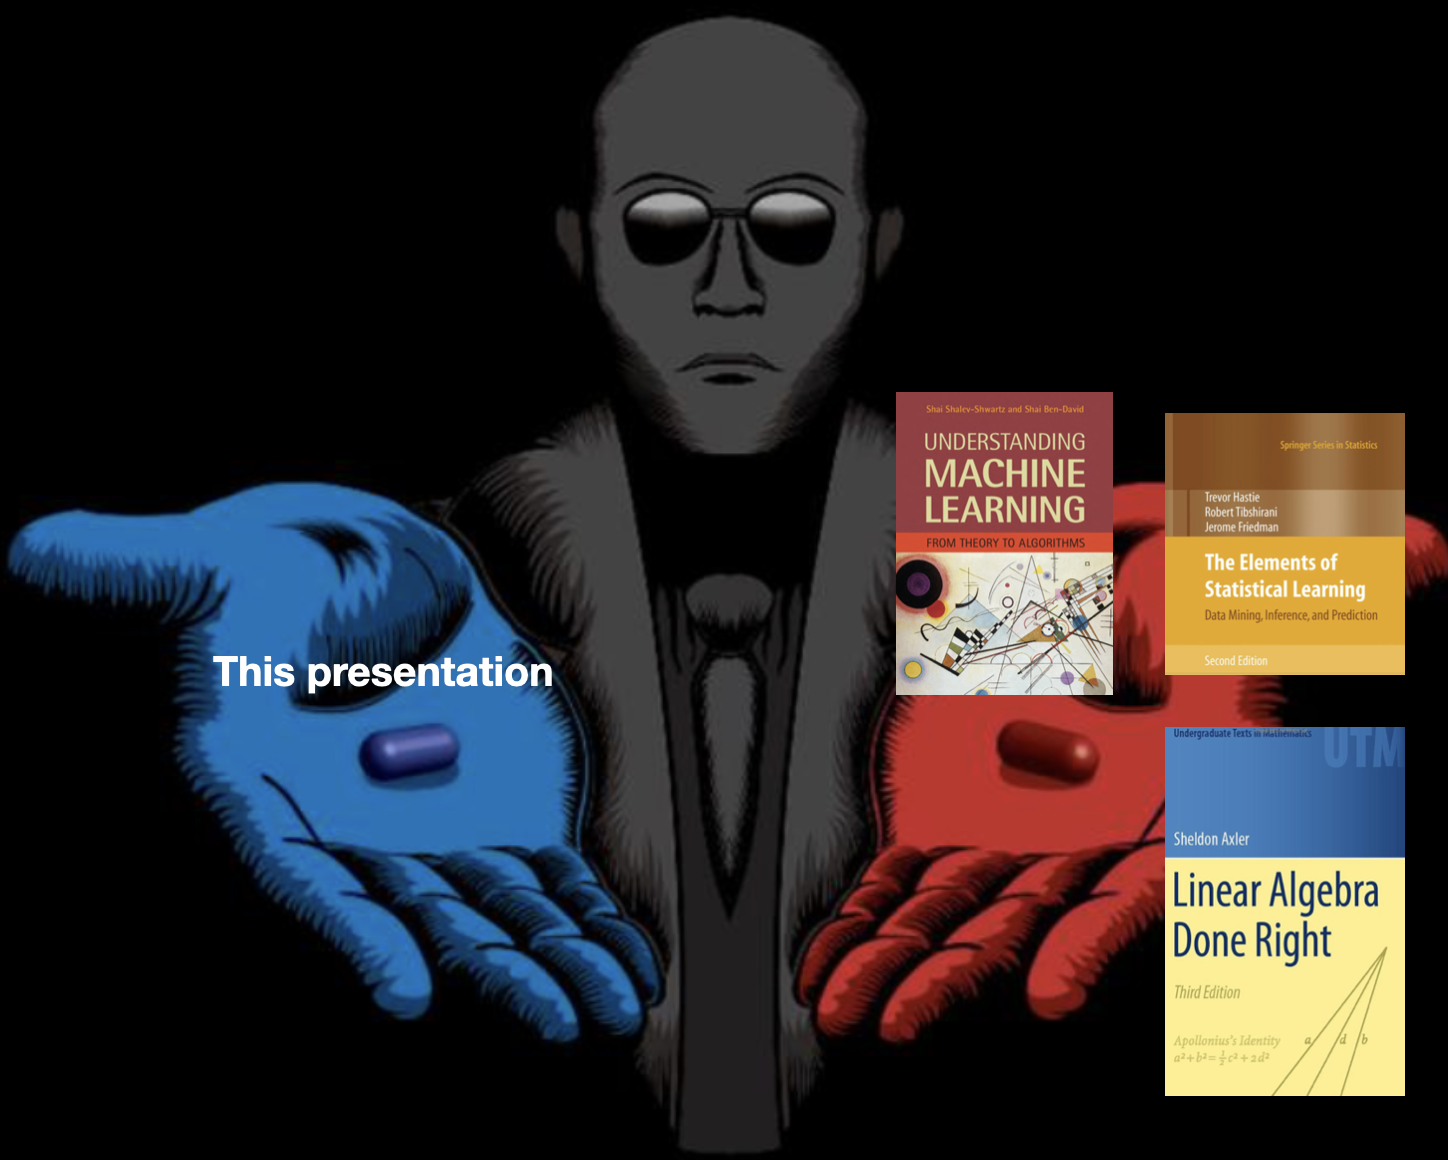
\includegraphics[width = .75\textwidth]{/Users/jacobblum/Desktop/cv_tex/figs/the_matrix.png}
        \caption{"You take the blue pill... the story ends, you wake up in your bed and believe whatever you want to believe. 
        You take the red pill... you stay in Wonderland, and I show you how deep the rabbit hole goes." - The Matrix (1999)}
    \end{figure}
\end{frame}


\begin{frame}
    \small{I cannot emphasize enough how important it is to \textit{learn by doing} here! The best way to learn about deep learning is to implement and train models using 
    open source databases like MNIST, fashion MNIST, and others!}

    Some other good resources include:
    \begin{itemize}
        \item 3Blue1brown's 4 part Neural Networks series (beginner)
        \item Free Towards Data Science tutorials (beginer + really helpful for the coding!) 
        \item Machine Learning and Simulation's youtube channel (intermediate)
        \item The Elements of Statistical Learning (Friedman, Tibshirani, and Hastie) (Advanced)
        \item Understanding Machine Learning: From Theory to Algorithms (Ben-David, Shalev-Shwartz) (Expert)
    \end{itemize}    

    \small{An understanding of linear-algebra, or better yet multi-linear algebra is essential to developming more advanced thinking about deep learning. In the future, 
    if you want to go on and study fields like Mathematics, any sort of physical science, engineering, or computer science, a strong grasp of this material will get you very far!}
    \end{frame}


\begin{frame}[plain]{Thank you!}

All the code from the demos and slides from this presentation is posted here: github.com/jacobblum/SFcomputervision


\end{frame}

\end{document}

